\documentclass[aspectratio=169]{beamer}

\usetheme{default}
\usepackage[utf8]{inputenc}
\usepackage[brazil]{babel}
\usepackage{tikz}
\usepackage{tabularx}
\usepackage{amsmath}
\usepackage{booktabs}
\usepackage{multirow}
\usepackage{graphicx}
\usepackage{hyperref}
\usepackage{amssymb}
\usepackage{colortbl}

% logos em presentation/imgs; figuras desta apresentação em ./figuras
\graphicspath{{../}{figuras/}}

\setbeamertemplate{footline}[frame number]
\setbeamertemplate{frametitle}[default][center]

\mode<presentation>{
\usetheme{Dresden}
\usecolortheme{seagull}
}

\setbeamertemplate{headline}{}

\definecolor{peeblue}{RGB}{1,123,165}
\definecolor{darkblue}{RGB}{0,65,115}

\setbeamercolor*{palette primary}{fg=black,bg=peeblue!80}
\setbeamercolor*{palette secondary}{fg=black,bg=peeblue!80!gray!80}
\setbeamercolor*{palette tertiary}{fg=black,bg=peeblue!100}
\setbeamercolor*{palette quaternary}{fg=black,bg=peeblue!110}

\usebackgroundtemplate
{%
    \begin{picture}(210,40)(-5,2)
    
\includegraphics[width=0.07\paperwidth,keepaspectratio]{imgs/pee-logo-short.png}
    \end{picture}%
}

\title{Reconhecimento Acústico de Alvos Submarinos no Dataset IARA}
\subtitle{Metadados Ambientais: Vento, Estado do Mar e os Erros de LARGE}
\author{Evandro Rocha}
\date{Novembro de 2026}

\institute
{
  Universidade Federal do Rio de Janeiro\\
  UFRJ / COPPE / PEE
}

\newcommand{\cahi}[1]{\cellcolor{green!30}\textbf{#1}}
\newcommand{\calo}[1]{\cellcolor{red!20}#1}
\newcommand{\camd}[1]{\cellcolor{yellow!35}#1}
\newcommand{\mix}{\texttt{MIX\_SMALL\_MEDIUM}}

\begin{document}

{
\usebackgroundtemplate{
    \begin{picture}(210,55)(-5,0)
    
\includegraphics[height=0.14\paperwidth,keepaspectratio]{imgs/pee-logo.png}
    \end{picture}%
    \begin{picture}(210,55)(-28,2)
    
\includegraphics[height=0.14\paperwidth,keepaspectratio]{imgs/coppe-logo.pdf}
    \end{picture}
}
\begin{frame}
  \bigskip\bigskip\bigskip\bigskip
  \titlepage
\end{frame}
}

\begin{frame}{Agenda da Apresentação}
  \footnotesize
  \setbeamercolor{block title}{bg=darkblue,fg=white}
  \setbeamercolor{block body}{bg=peeblue!8,fg=black}
  \setbeamertemplate{section in toc}{%
    \vspace{0.14cm}%
    \leavevmode%
    \tikz[baseline=-0.65ex]\node[circle,fill=peeblue,text=white,inner sep=0pt,font=\tiny\bfseries,minimum size=1.35em]{\inserttocsectionnumber};%
    \hspace{0.35em}%
    \inserttocsection\par%
  }
  \begin{columns}[t]
      \begin{column}{0.6\textwidth}
          \begin{block}{\small\textbf{Metadados Ambientais}}
              \tableofcontents
          \end{block}
      \end{column}
  \end{columns}
\end{frame}

\begin{frame}{Resumo}
    \footnotesize
    \begin{block}{\small Pergunta: os metadados ambientais do IARA explicam os erros de LARGE? Dá para usá-los?}
        \scriptsize
        \begin{enumerate}
            \setlength{\itemsep}{3pt}
            \item \textbf{Metadados públicos são poucos:} chuva, vento, estado do mar (estação próxima) e CPA. \textbf{Sem data, hora e observatório}; dados brutos só por solicitação ao PMPAS-BS.
            \item \textbf{Os LARGE foram gravados com o mar mais calmo} (mar $\leq$ 2 em 58\% das gravações, contra 43--46\% de SMALL e MEDIUM).
            \item \textbf{A MLP erra mais LARGE com o mar agitado:} com CPA 81 $\rightarrow$ 69\%; sem CPA 54 $\rightarrow$ 45\%.
            \item \textbf{Augmentation com ruído real de mar agitado não ajudou:} recall de LARGE 67,7 $\rightarrow$ 66,1\% no mix\_small\_medium e 67,7 $\rightarrow$ 65,4\% nas 4 classes (split por navio, não significativo). O ruído apaga parte do grave dos LARGE.
        \end{enumerate}
    \end{block}
\end{frame}

%===========================================
\section{Que Metadados Existem}

\begin{frame}
    \centering
    \huge Que Metadados Existem
\end{frame}

\begin{frame}{O que o IARA Publica}
    \footnotesize
    \begin{columns}[t]
        \column{0.5\textwidth}
        \begin{block}{\small Zenodo (DOI 10.5281/zenodo.15777429)}
            \scriptsize
            \begin{itemize}
                \setlength{\itemsep}{1pt}
                \item Áudios já recortados (A.zip a H.zip, 31,6 GB, 1825 gravações de 2 a 5 min).
                \item Planilha \texttt{iara.xlsx}; licença CC BY-NC 4.0.
            \end{itemize}
        \end{block}
        \begin{block}{\small Por gravação}
            \scriptsize
            \begin{itemize}
                \setlength{\itemsep}{1pt}
                \item Chuva, vento e estado do mar (\textbf{estação meteorológica próxima}; o estado do mar é estimado pelo vento).
                \item Instante do CPA (só A e C).
                \item Navio: nome, tipo, comprimento, MMSI, IMO.
            \end{itemize}
        \end{block}
        \column{0.48\textwidth}
        \begin{alertblock}{\small O que não existe}
            \scriptsize
            \begin{itemize}
                \setlength{\itemsep}{1pt}
                \item \textbf{Data e hora} da gravação (``Recording time'' é a duração).
                \item \textbf{Observatório} de origem.
                \item Gravações contínuas e AIS.
            \end{itemize}
        \end{alertblock}
        \begin{block}{\small PMPAS-BS / SIMMAO}
            \scriptsize
            Os dados brutos são do projeto de monitoramento da Petrobras. O portal SIMMAO mostra dados processados (mapas de ruído, espectros, densidade de tráfego AIS) e tem um formulário de \textbf{solicitação de dados para fins científicos}.
        \end{block}
    \end{columns}
    \begin{alertblock}{Leitura}
        \scriptsize
        Sem data e observatório, não dá para testar efeitos de época ou de equipamento. Vale pedir esses metadados aos autores: são bem mais fáceis de obter que o áudio contínuo.
    \end{alertblock}
\end{frame}

%===========================================
\section{Condições de Gravação}

\begin{frame}
    \centering
    \huge Condições de Gravação
\end{frame}

\begin{frame}{Os LARGE Foram Gravados com o Mar Mais Calmo}
    \begin{columns}[c]
        \column{0.58\textwidth}
        \centering
        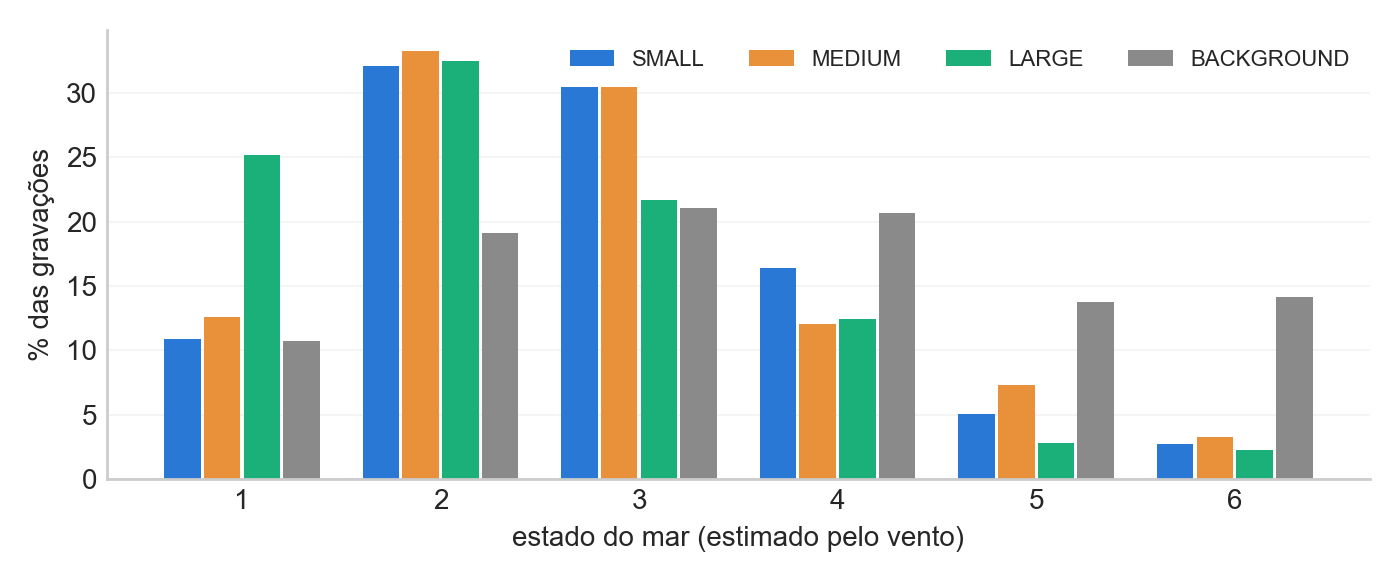
\includegraphics[width=\textwidth]{mar_por_classe.png}
        \column{0.4\textwidth}
        \begin{block}{\small Por gravação}
            \tiny
            \centering
            \setlength{\tabcolsep}{3pt}
            \begin{tabular}{lccc}
            \toprule
             & Vento & Mar calmo & Chuva \\
             & (m/s) & (estado $\leq$ 2) & \\
            \midrule
            SMALL & 4,8 & 43\% & 8\% \\
            MEDIUM & 4,7 & 46\% & 5\% \\
            LARGE & \cahi{3,8} & \cahi{58\%} & 7\% \\
            BACKGROUND & 6,8 & 30\% & \calo{42\%} \\
            \bottomrule
            \end{tabular}
        \end{block}
    \end{columns}
    \vspace{0.05cm}
    \begin{alertblock}{Leitura}
        \scriptsize
        Por navio, a diferença é significativa entre LARGE e os navios $<$ 100 m (p $<$ 0,001), mas não entre SMALL e MEDIUM (p = 0,71). \textbf{É um viés da base}: com condições iguais, a separação entre as classes provavelmente seria um pouco menor. Chuva quase só aparece no BACKGROUND, que foi escolhido em condições variadas.
    \end{alertblock}
\end{frame}

\begin{frame}{O BACKGROUND Cobre Mar Agitado}
    \footnotesize
    \begin{columns}[t]
        \column{0.55\textwidth}
        \begin{block}{\small BACKGROUND (subconjunto E): estado do mar $\times$ chuva}
            \tiny
            \centering
            \setlength{\tabcolsep}{4pt}
            \begin{tabular}{lcccc}
            \toprule
            Estado do mar & Sem chuva & Com chuva & Total \\
            \midrule
            1 & 25 & 3 & 28 \\
            2 & 25 & 25 & 50 \\
            3 & 25 & 30 & 55 \\
            4 & \cahi{25} & 29 & 54 \\
            5 & \cahi{25} & 11 & 36 \\
            6 & \cahi{25} & 12 & 37 \\
            7 & \cahi{1} & 0 & 1 \\
            \bottomrule
            \end{tabular}
        \end{block}
        \column{0.43\textwidth}
        \begin{block}{\small Desenho proposital}
            \scriptsize
            \begin{itemize}
                \setlength{\itemsep}{1pt}
                \item 25 gravações sem chuva \textbf{em cada estado do mar} de 1 a 6.
                \item Vento de 1,3 a 20 m/s.
                \item Nenhum navio num raio de 10 km.
                \item 76 fundos sem chuva com mar $\geq$ 4; 50 com mar $\leq$ 2.
            \end{itemize}
        \end{block}
    \end{columns}
    \begin{alertblock}{Leitura}
        \scriptsize
        Há material para ``sujar'' gravações LARGE de mar calmo com ruído real de mar agitado. Os LARGE, ao contrário, têm só 29 gravações com mar 5 ou 6.
    \end{alertblock}
\end{frame}

\begin{frame}{A MLP Erra Mais LARGE com o Mar Agitado}
    \begin{columns}[c]
        \column{0.58\textwidth}
        \centering
        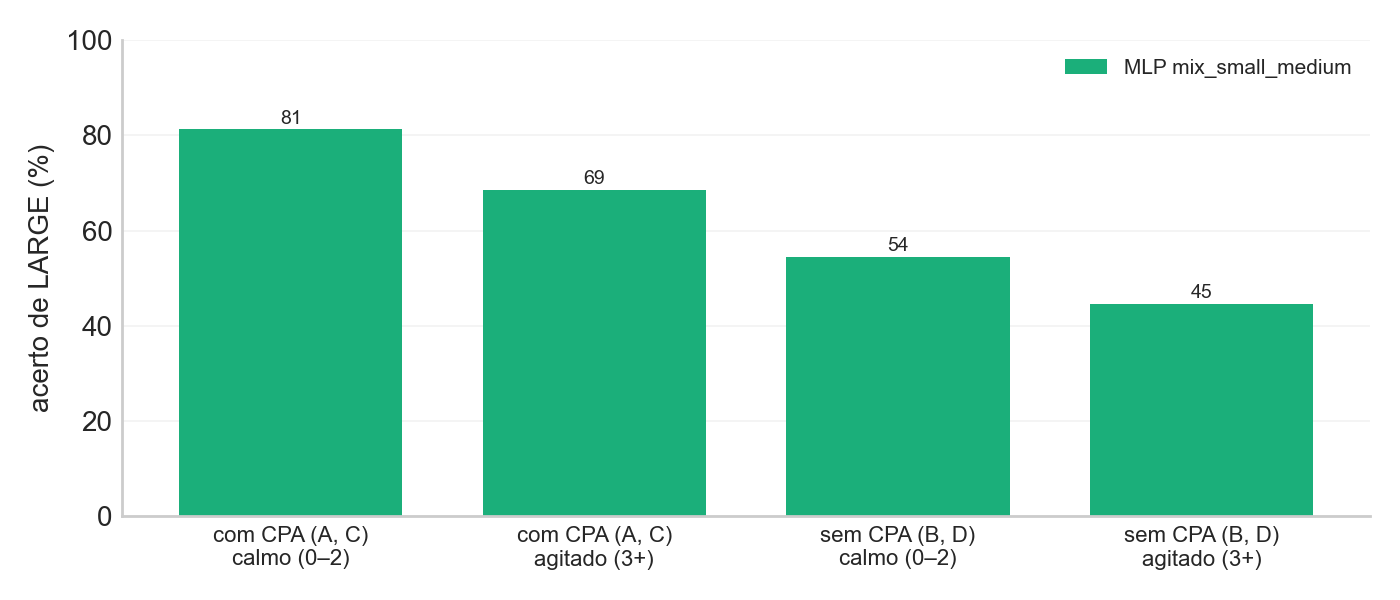
\includegraphics[width=\textwidth]{large_cpa_mar.png}

        {\tiny MLP mix\_small\_medium (NB40), split por navio.\par}
        \column{0.4\textwidth}
        \begin{block}{\small Faixa 31--86 Hz (dB acima do fundo)}
            \tiny
            \centering
            \begin{tabular}{lcc}
            \toprule
             & Calmo & Agitado \\
            \midrule
            Com CPA & 8,0 & 7,1 \\
            Sem CPA & 7,0 & 5,8 \\
            \bottomrule
            \end{tabular}
        \end{block}
        \begin{block}{\small \texttt{MIX\_SMALL\_MEDIUM} com CPA}
            \tiny
            Calmo 77\% $\rightarrow$ agitado 75\%: quase não sofre.
        \end{block}
    \end{columns}
    \vspace{0.05cm}
    \begin{alertblock}{Leitura}
        \scriptsize
        \textbf{O mar agitado tira $\sim$10 pontos do acerto de LARGE, com ou sem CPA}; o pior caso (sem CPA e agitado) acerta só 45\%. O ruído do mar sobe e o grave do navio se destaca menos do fundo. Vento e estado do mar vêm de estação próxima, não do local.
    \end{alertblock}
\end{frame}

%===========================================
\section{Augmentation com Mar Agitado}

\begin{frame}
    \centering
    \huge Augmentation com Mar Agitado
\end{frame}

\begin{frame}{Como Foi Feito}
    \footnotesize
    \begin{columns}[t]
        \column{0.52\textwidth}
        \begin{block}{\small Procedimento}
            \scriptsize
            \begin{itemize}
                \setlength{\itemsep}{2pt}
                \item \textbf{Áudio} de cada gravação LARGE + gravação de BACKGROUND sem chuva com mar $\geq$ 4; razão sinal/fundo sorteada entre 0 e 20 dB; LOFAR recalculado igual ao do pipeline.
                \item No treino, cada LARGE ganha \textbf{uma} versão misturada, com fundo do \textbf{treino} daquele fold (sem vazamento). Teste: LOFAR original.
                \item Mesma MLP h32-16 e folds, nos dois splits: no mix\_small\_medium e no problema original de 4 classes.
                \item O LOFAR original não é alterado: pastas novas.
            \end{itemize}
        \end{block}
        \column{0.46\textwidth}
        \begin{block}{\small Variantes}
            \scriptsize
            \begin{itemize}
                \setlength{\itemsep}{2pt}
                \item \textbf{agitado:} fundo de mar $\geq$ 4 (76 gravações).
                \item \textbf{calmo (controle):} mesma mistura com fundo de mar $\leq$ 2 (50 gravações).
                \item \textbf{dupL (controle):} cópia idêntica do LARGE (mais exemplos, sem ruído).
            \end{itemize}
        \end{block}
        \begin{alertblock}{\small Por que os controles}
            \scriptsize
            Separam o efeito do \emph{mar agitado} do efeito de ter mais LARGE ou de qualquer fundo.
        \end{alertblock}
    \end{columns}
\end{frame}

\begin{frame}{Resultado: Nenhuma Variante Ajuda}
    \footnotesize
    \begin{table}
    \centering
    \scriptsize
    \setlength{\tabcolsep}{4pt}
    \begin{tabular}{lccccc}
    \toprule
     & \multicolumn{4}{c}{Split por navio} & Split por gravação \\
    \cmidrule(lr){2-5}\cmidrule(lr){6-6}
    Variante & ACC & \texttt{MIX} & LARGE & BACKGROUND & ACC \\
    \midrule
    Sem augmentation & 74,6 & 76,2 & 67,7 & 79,9 & 78,1 \\
    dupL (controle) & 75,4 & 78,2 & 67,1 & 81,0 & 78,3 \\
    Fundo calmo (controle) & 74,9 & 79,3 & \calo{64,4} & 80,8 & 77,5 \\
    \textbf{Fundo agitado} & 74,3 & 78,0 & \calo{66,1} & 78,8 & 77,2 \\
    \bottomrule
    \end{tabular}
    \end{table}
    {\tiny Média de 10 folds. Teste F 5x2cv contra ``sem augmentation'': todos com p $>$ 0,05 (menor p = 0,07).\par}
    \vspace{0.1cm}
    \begin{alertblock}{Leitura}
        \scriptsize
        \textbf{Nenhuma variante melhora o modelo.} Misturar fundo tira um pouco de recall de LARGE (agitado $-$1,6; calmo $-$3,2 pontos no split por navio; não significativo) e dá um pouco a \texttt{MIX}. Como o fundo \emph{calmo} faz o mesmo, \textbf{não é efeito do mar agitado}: é o efeito de mostrar LARGE com o grave ``diluído''.
    \end{alertblock}
\end{frame}

\begin{frame}{Os LARGE de Mar Agitado Não Melhoraram}
    \centering
    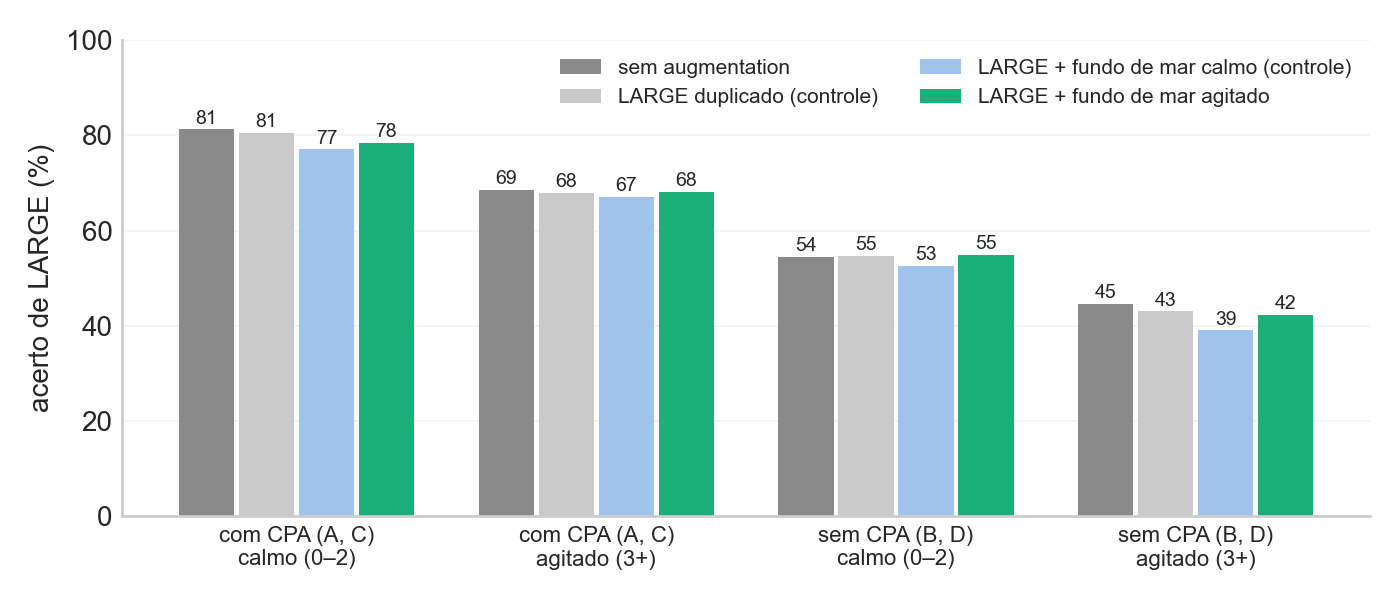
\includegraphics[width=0.8\textwidth]{large_cpa_mar_aug.png}

    {\tiny Split por navio.\par}
    \vspace{0.05cm}
    \begin{alertblock}{Leitura}
        \scriptsize
        Onde o efeito era esperado (mar agitado), o acerto fica igual ou cai: com CPA 69 $\rightarrow$ 68\%, sem CPA 45 $\rightarrow$ 42\%. \textbf{Interpretação provável:} somar ruído apaga parte do grave que diferencia o LARGE; o exemplo aumentado fica parecido com um navio $<$ 100 m (medido adiante). Quando o grave some do LOFAR, a informação não está lá para ser aprendida.
    \end{alertblock}
\end{frame}

\begin{frame}{E no Problema Original de 4 Classes?}
    \footnotesize
    \begin{table}
    \centering
    \scriptsize
    \setlength{\tabcolsep}{3.5pt}
    \begin{tabular}{lcccccc}
    \toprule
     & \multicolumn{5}{c}{Split por navio} & Split por gravação \\
    \cmidrule(lr){2-6}\cmidrule(lr){7-7}
    Variante & ACC & SMALL & MEDIUM & LARGE & BACKGROUND & ACC \\
    \midrule
    Sem augmentation & 58,3 & 49,8 & 34,5 & 67,7 & 81,1 & 67,8 \\
    dupL (controle) & 58,3 & 47,5 & 36,9 & 67,6 & 81,1 & 68,1 \\
    Fundo calmo (controle) & 57,6 & 49,7 & 36,8 & \calo{63,3} & 80,4 & 67,3 \\
    \textbf{Fundo agitado} & 57,7 & 48,9 & 36,4 & \calo{65,4} & 79,9 & 67,0 \\
    \bottomrule
    \end{tabular}
    \end{table}
    {\tiny Mesma MLP h32-16 e mesmos folds da MLP LOFAR de 4 classes do NB29; mesmas cópias aumentadas. Média de 10 folds. Teste F 5x2cv contra ``sem augmentation'': todos com p $>$ 0,05 (menor p = 0,09). Split por gravação, recall de LARGE: 71,2 (sem) / 70,0 (dupL) / 63,6 (calmo) / 67,4 (agitado).\par}
    \vspace{0.1cm}
    \begin{alertblock}{Leitura}
        \scriptsize
        \textbf{Mesmo resultado do mix\_small\_medium.} Repetir os LARGE (dupL) não muda nada; misturar fundo, calmo ou agitado, tira recall de LARGE (2--4 pontos no split por navio, 4--8 no split por gravação) e os erros vão para SMALL/MEDIUM. Os LARGE gravados com mar agitado também não melhoram (com CPA: 68 $\rightarrow$ 67\%; sem CPA: 43 $\rightarrow$ 42\%).
    \end{alertblock}
\end{frame}

\begin{frame}{O Ruído Apaga o Grave dos LARGE?}
    \footnotesize
    \begin{columns}[t]
        \column{0.5\textwidth}
        \begin{block}{\small Queda em 31--86 Hz (cópia $\times$ original)}
            \scriptsize
            \centering
            \setlength{\tabcolsep}{4pt}
            \begin{tabular}{lcc}
            \toprule
            Razão sinal/fundo & Mar agitado & Mar calmo \\
            \midrule
            0--5 dB & \calo{$-$30\%} & $-$19\% \\
            5--10 dB & $-$19\% & $-$10\% \\
            10--15 dB & $-$9\% & $-$5\% \\
            15--20 dB & $-$4\% & $-$2\% \\
            \midrule
            Todas & $-$12\% & $-$6\% \\
            \bottomrule
            \end{tabular}

            \vspace{0.1cm}
            {\tiny Mediana por cópia; 2288 cópias de 572 LARGE por fundo; LOFAR que a MLP recebe.\par}
        \end{block}
        \column{0.48\textwidth}
        \begin{block}{\small Cópias que parecem navio $<$ 100 m}
            \scriptsize
            Grave (31--86 Hz) abaixo da mediana de SMALL+MEDIUM:
            \begin{itemize}
                \setlength{\itemsep}{1pt}
                \item LARGE originais: 24\%
                \item cópias com mar agitado: 38\%
                \item cópias com mar agitado e 0--5 dB: \textbf{54\%}
            \end{itemize}
            A banda dos navios $<$ 100 m (90--221 Hz) quase não muda com mar agitado ($-$0,4\%).
        \end{block}
    \end{columns}
    \begin{alertblock}{Leitura}
        \scriptsize
        \textbf{O mecanismo existe:} o ruído levanta o fundo local (TPSW) e o grave que identifica o LARGE sobressai menos; com muito ruído, metade das cópias fica com o grave de um navio $<$ 100 m. \textbf{Mas não explica tudo:} o mar calmo apaga menos grave e tirou um pouco mais de recall (diferença não significativa). Como o ruído é somado no áudio, trocar LOFAR por MEL provavelmente não resolveria.
    \end{alertblock}
\end{frame}


%===========================================
\section{Como Usar os Metadados}

\begin{frame}
    \centering
    \huge Como Usar os Metadados
\end{frame}

\begin{frame}{Usar Vento e Estado do Mar Direto no Modelo?}
    \footnotesize
    \begin{alertblock}{\small Risco: atalho}
        \scriptsize
        Hoje os modelos recebem só o LOFAR, que remove o nível de fundo (TPSW) e o volume (normalização). Pôr vento e estado do mar como entradas é fácil, mas como os LARGE foram gravados com mar mais calmo, o modelo aprenderia \textbf{``mar calmo $\rightarrow$ LARGE''}: melhora o número no IARA e piora no mundo real.
    \end{alertblock}
    \begin{block}{\small Usos mais seguros}
        \scriptsize
        \begin{enumerate}
            \setlength{\itemsep}{2pt}
            \item \textbf{Augmentation direcionado:} o metadado só escolhe o ruído, não entra no modelo.
            \item \textbf{Abstenção:} com mar agitado e grave fraco, responder ``inconclusivo''.
            \item \textbf{Medir o ruído pelo próprio áudio} (nível antes da normalização), sem depender de estação meteorológica.
            \item \textbf{Reportar por condição:} mar calmo $\times$ agitado, com $\times$ sem CPA.
        \end{enumerate}
    \end{block}
\end{frame}

%===========================================
\section{Conclusões}

\begin{frame}
    \centering
    \huge Conclusões
\end{frame}

\begin{frame}{Conclusões}
    \footnotesize
    \begin{block}{\small O que os metadados mostram}
        \scriptsize
        \begin{enumerate}
            \setlength{\itemsep}{2pt}
            \item \textbf{Ajudam a entender os erros, não a corrigi-los:} mar agitado e falta de CPA explicam boa parte dos erros de LARGE (45\% de acerto quando se juntam).
            \item \textbf{Viés de condição:} os LARGE foram gravados com o mar mais calmo; os resultados de LARGE no IARA são provavelmente um pouco otimistas.
            \item \textbf{Augmentation com mar agitado não ajudou}, nem no mix\_small\_medium nem nas 4 classes; misturar qualquer fundo tira um pouco de recall de LARGE, porque o ruído apaga parte do grave.
            \item \textbf{Não usar vento e estado do mar como entrada} (atalho ``mar calmo $\rightarrow$ LARGE''). Usar para reportar por condição e para abstenção.
        \end{enumerate}
    \end{block}
    \begin{alertblock}{\small Próximo passo sugerido}
        \scriptsize
        Pedir aos autores / PMPAS-BS (formulário do SIMMAO): \textbf{data, hora e observatório} de cada gravação do IARA (testar época e equipamento) e, se possível, \textbf{áudio contínuo + AIS} para ampliar os navios abaixo de 100 m.
    \end{alertblock}
\end{frame}


\end{document}
